\chapter{User manual}


\section{The web interface}
You can connect to your PDR instance using any web browser. Just navigate to your server and enter your username and password.

\subsection{Login}
\begin{figure}[h]
	\centering
	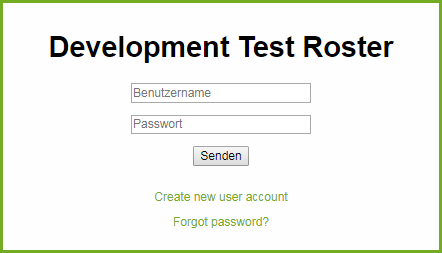
\includegraphics{{images/en_GB/login.php}.png}
	\caption{Login page}
\end{figure}
The login page shows the name of the application. You are prompted to enter your username and password.
If you do not have an account yet, you can create one. Just follow the link.
If you have an account, but forgot about your password, or want to change it, you can click on "Lost password?".

\subsection{Lost password}
\begin{figure}[h]
	\centering
	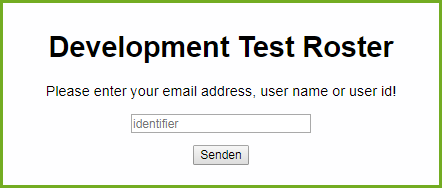
\includegraphics{{images/en_GB/lost_password.php}.png}
	\caption{Lost password page}
\end{figure}
The lost password page shows the name of the application. You are prompted to enter either your username, id or your email-address at your option.
After you submit the form, an email is sent to your stored email address.
In that email you will find a link. That link will lead you to the password change page.
\subsubsection{Lost password recovery}
\begin{figure}[ph]
	\centering
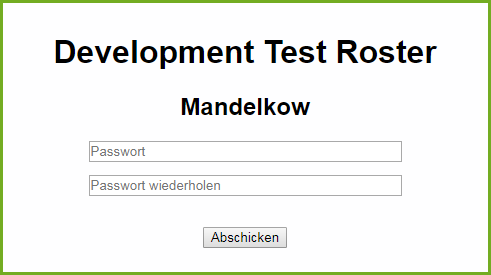
\includegraphics[width=0.4\linewidth]{{images/en_GB/reset-lost-password.php}.png}
	\caption{Lost password recovery page}
\end{figure}
The lost password recovery page shows the name of the application and your user name. You are prompted to enter a new password twice.

\subsection{Create new user account}
\begin{figure}[ph]
	\centering
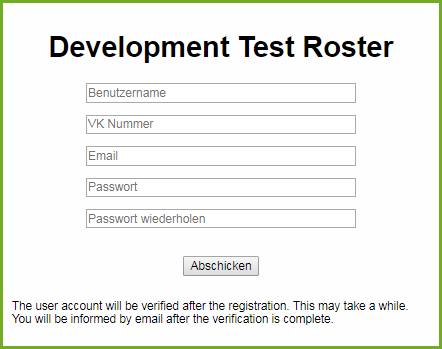
\includegraphics[width=0.4\linewidth]{{images/en_GB/register.php}.png}
	\caption{Register new user page}
\end{figure}
New users can only be created for existing employees. New employees are created by an administrator. Choose a user name, enter your employee id and your email. And enter a password twice.

The account will be inactive until an administrator activates it. The administrator is informed via email regarding the registration.


\subsection{Navigation}
\begin{figure}[ph]
	\centering
	
\includegraphics[width=0.8\linewidth]{{images/en_GB/navigation}.png}
	\caption{Navigation bar}
\end{figure}
By default, the PDR web interface opens to your a menu containing 5 tiles.
You can navigate to:
\begin{itemize}
\item Roster week table view
\item Roster daily view
\item Roster employee view
\item Overtime 
\item Absence
\end{itemize}

\subsubsection{The navigation bar}
In the top there is a navigation bar containing hyperlinks to nearly all the pages of PDR. Hover the mouse over an entry to open the submenus.

\subsubsection{Roster week table view}
\begin{figure}[h]
	\centering
	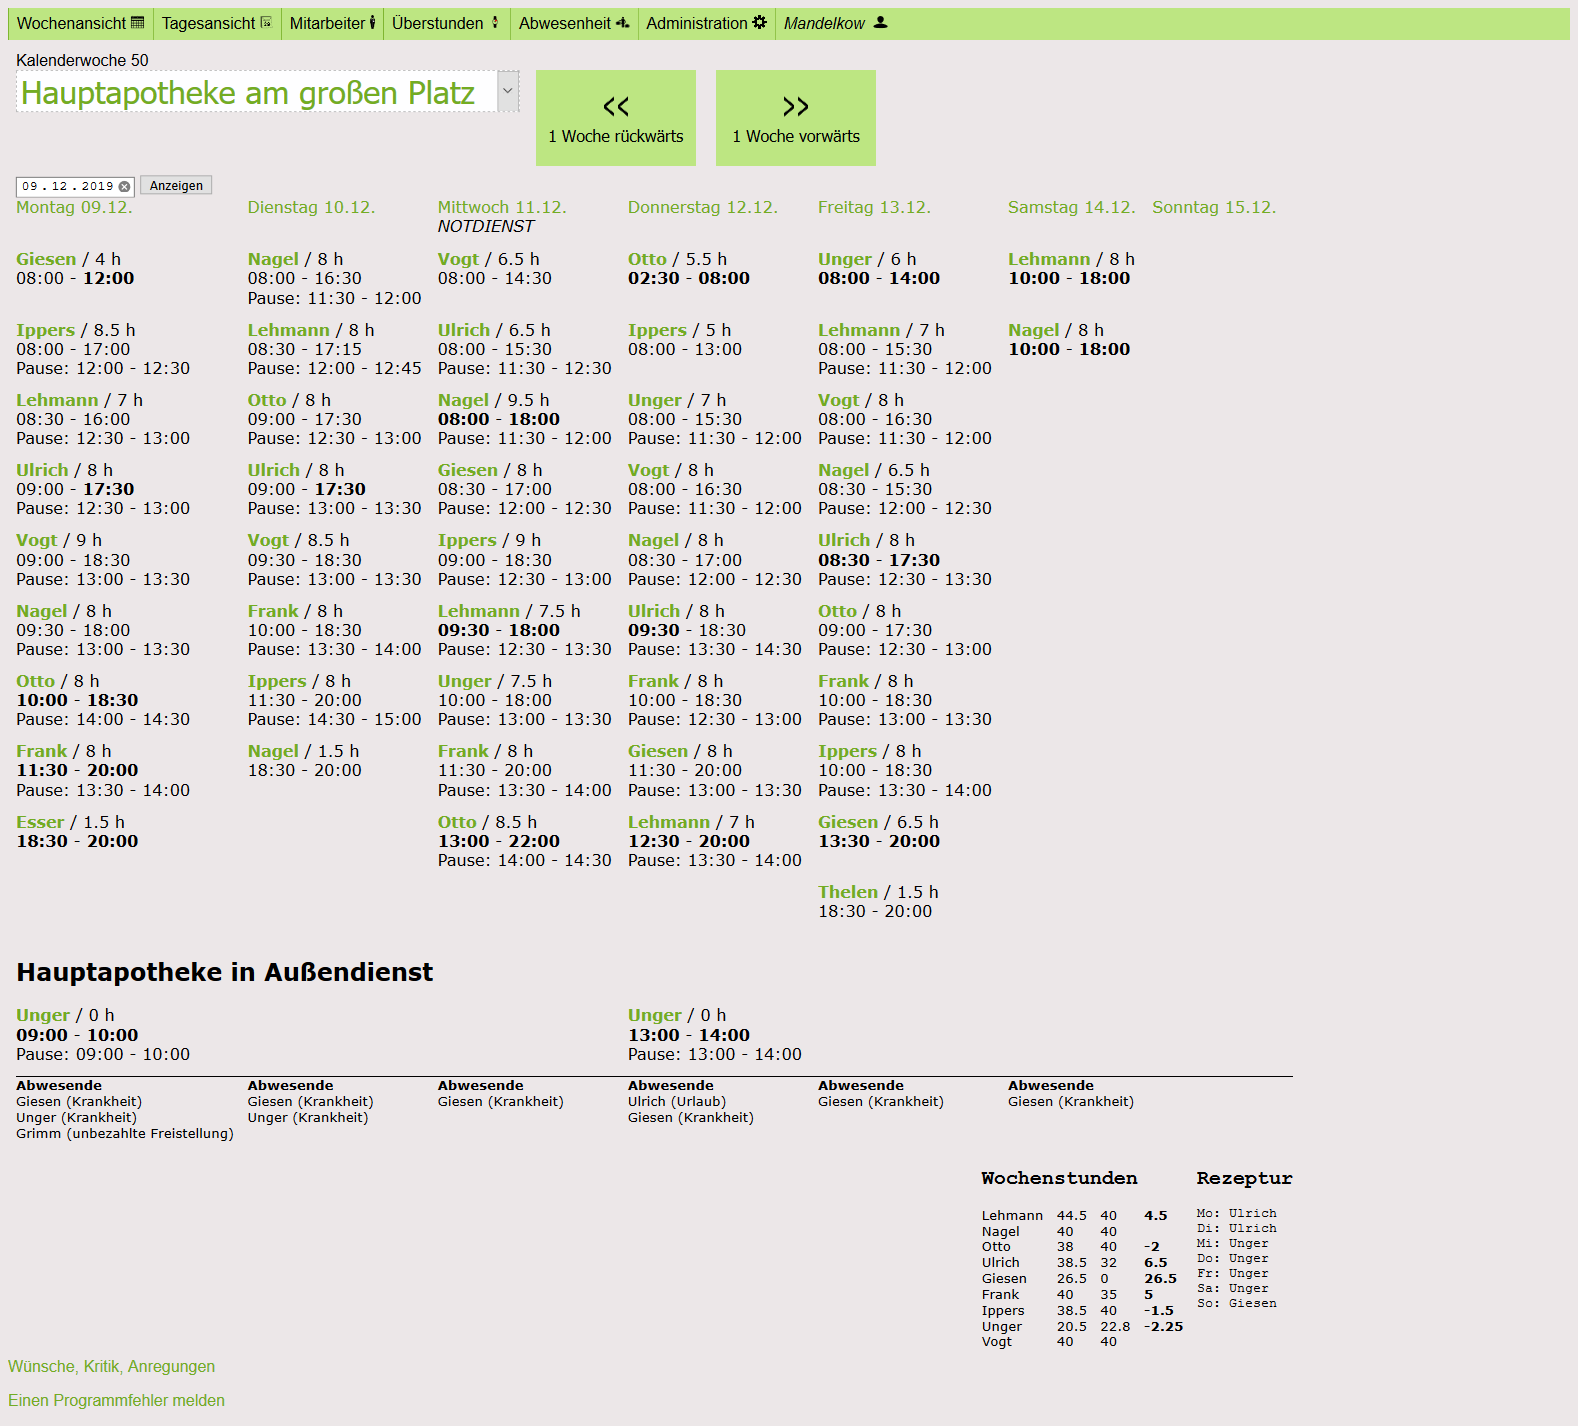
\includegraphics[width=0.8\linewidth]{{images/en_GB/roster-week-table.php}.png}
	\caption{Roster week table view, excerpt without task rotation and weekly working hours}
\end{figure}


\subsubsection{Roster daily view}
\subsubsection{Roster employee view}
\subsubsection{Overtime}
\subsubsection{Absence}
There are four views to the absence data.
\begin{itemize}
\item Employee view readonly
\item Employee view edit
\item Monthly table
\item Year overview
\end{itemize}
In the \emph{Employee view readonly} there is a select element to choose the employee to view. There is a button to switch to the edit view.
And there is a table containing the absence data. The columns are start and end of the absence, reason of absence and number of days.
There is a distinct list of possible reasons ( vacation,
        remaining holiday,
       sickness,
        sickness of child,
        unpaid leave of absence,
        paid leave of absence,
        parental leave and
        maternity leave).
The number of days of absence is calculated for a 5 day week. Absences on saturdays and sundays are registered but not counted. The same applys for holidays.